\chapter{معماری پروژه}

همانطور که در {\ref{fig:architecture}} می‌بینید این پروژه از معماری میکروسرویس بهره می‌برد.
در این فصل ابتدا به معرفی کلی هر سرویس و سپس نگاهی دقیق به عملکرد هر سرویس می‌اندازیم.

\begin{figure}[htbp]
    \centering
    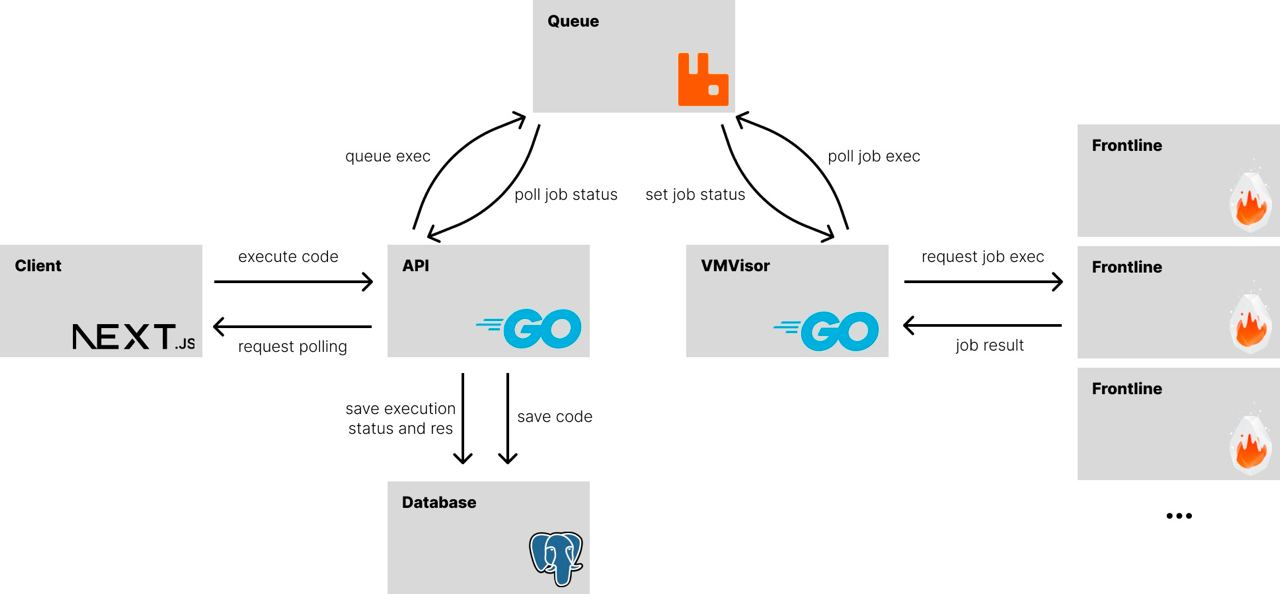
\includegraphics[width=1\textwidth]{./3-Design/design.jpg}
    \caption{معماری پروژه}
    \label{fig:architecture}
\end{figure}

\newpage

همانطور که در شکل و جدول مشاهده می‌کنید پروژه از ۴ سرویس اصلی تشکیل شده است.
درخواست از کلاینت شروع شده پس از طی کردن API و VMVisor به Frontline می‌رسد.
پیش تر اشاره کردیم که Frontline یه Web API است که درون vm در حال اجراست.
Frontline در اصل یک Web API است که با پروسه فرزند کامپایلر زبان های مختلف را فراخوانی کرده و خروجی را بر می‌گرداند.


\begin{table}[hb]
    \centering
    \caption{لیست سرویس ها}
    \label{table:services}
    \begin{tabular}{|c|c|}
        \hline
        سرویس ها  & توضیحات                                                                \\
        \hline

        API       & سرویس REST API است که وظیفه صحبت با دیتابیس و پاسخ به کلاینت را دارد   \\
        \hline

        VMVisor   & مدیریت VM های ساخته و دریافت و تغییر وضعیت درخواست های اجرا روی صف     \\
        \hline

        Frontline & درون هر VM در حال اجراست و توسط پروسه فرزند کامپایلر زبان را صدا می‌زند \\
        \hline


        Client    & کلاینت وطیفه نمایش رابط کاربری و ادیتور را دارد                        \\
        \hline
    \end{tabular}
\end{table}


مهم ترین سرویس این پروژه VMVisor است که وظیفه مدیریت vm ها را بر عهده دارد.
این پروژه از Firecracker استفاده می‌کند و مجموعه ای از vm ها را مدیریت و به آن ها وظیفه ای برای اجرا می‌سپارد.


ارتباط بین API و VMVisor به صورت آستکرون توسط انتقال پیام در صف است.
در RabbitMQ دو صف وجود دارد. صف درخواست اجرا و صف وضعیت اجرا.
در صف درخواست اجرا سرویس API کدی که کلاینت ارسال کرده را روی صف قرار می‌دهد
و VMVisor این درخواست را از صف بر‌می‌دارد.
صف دیگر وضعیت اجرا است که VMVisor خروجی Frontline را روی صف قرار می‌دهد و API به آن گوش می‌دهد و روی پایگاه داده می‌نویسد.

وظیفه API عملیات های CRUD(create read update delete) است و اولین درگاهی است که کلاینت با آن در ارتباط است.
همچنین وظیفه قرار دادن درخواست اجرا در صف و گوش دادن به صف وضعیت اجرا و نوشتن آن روی پایگاه داده را برعهده دارد.
از دیگر وظیفه های این سرویس مدیریت کاربران و پروژه های آن ها است.
این سرویس خود پتانسیل شکسته شدن به میکروسرویس های کوچک تر را دارد ولی در این پروژه این تصمیم گرفته نشده است.

کلاینت هم بخش مهم دیگری است که رابط کاربری سیستم با نرم افزار است. کاربر امکان ساخت پروژه جدید و ویرایش آن در مرورگر را دارد.
رابط کاربری این پروژه در Figma طراحی شده و توسط کتابخانه React دیزاین سیستم طراحی شده و کامپوننت های مختلف در کنار هم قرار گرفته اند.

در ادامه به معرفی دقیق تر هر سرویس و ارتباطش با سایرین می‌پردازیم.